\documentclass[a4paper,twoside]{ctexart}
\usepackage{geometry}
\geometry{margin=1cm,vmargin={0pt,1cm}}
\setlength{\topmargin}{-2cm}
\setlength{\paperheight}{23cm}
\setlength{\paperwidth}{18cm}
\setlength{\textheight}{19.6cm}
\setlength{\textwidth}{15cm}
\usepackage{makecell}
\usepackage{fancyhdr}
\usepackage{siunitx}
\usepackage{amssymb}
\usepackage{indentfirst}
\setlength{\parindent}{0.5em}

\pagenumbering{arabic}

% useful packages.
\usepackage{multirow}
\usepackage{caption}
\usepackage{mathrsfs}
\usepackage{amsfonts}
\usepackage{amsmath}
\usepackage{amsthm}
\usepackage{enumerate}
\usepackage{xcolor,graphicx,float,subfigure}
\usepackage{epstopdf}
\usepackage{multicol}
\usepackage{fancyhdr}
\usepackage{layout}
\usepackage{listings}
\usepackage{diagbox}
\lstset{
    basicstyle=\tt,
    numbers=left,
    rulesepcolor=\color{red!20!green!20!blue!20},
    escapeinside=``,
    xleftmargin=2em,xrightmargin=2em, aboveskip=1em,
    framexleftmargin=1.5mm,
    frame=shadowbox,
    backgroundcolor=\color[RGB]{245,245,244},
    keywordstyle=\color{blue}\bfseries,
    identifierstyle=\bf,
    numberstyle=\color[RGB]{0,192,192},
    commentstyle=\it\color[RGB]{96,96,96},
    stringstyle=\rmfamily\slshape\color[RGB]{128,0,0},
    showstringspaces=false
}
\usepackage[colorlinks,linkcolor=blue]{hyperref}
\usepackage{xcolor}
\usepackage{cite}
\usepackage[numbers,sort&compress]{natbib}
\setcitestyle{open={},close={}}
%\usepackage{natbibspacing}
%\renewcommand{\refname}{}
\usepackage{anyfontsize}

% 中文定理环境

\newtheorem{definition}{定义}[section]
\newtheorem{example}{例}[section]
\newtheorem{remark}{注}[section]
\newtheorem{lemma}[definition]{引理}
\newtheorem{theorem}[definition]{定理}
\newtheorem{proposition}[definition]{命题}
\newtheorem{corollary}[definition]{推论}
\newenvironment{solution}{\begin{proof}[\indent\bf 解]}{\end{proof}}
\renewcommand{\proofname}{\bf 证明}

% % English theorem environment
% \newtheorem{theorem}{Theorem}[section]
% \newtheorem{lemma}[theorem]{Lemma}
% \newtheorem{proposition}[theorem]{Proposition}
% \newtheorem{corollary}[theorem]{Corollary}
% \newtheorem{definition}{Definition}[section]
% \newtheorem{remark}{Remark}[section]
% \newtheorem{example}{Example}[section]
% \newenvironment{solution}{\begin{proof}[Solution]}{\end{proof}}

% some common command
\newcommand{\dif}{\mathrm{d}}
\newcommand{\avg}[1]{\left\langle #1 \right\rangle}
\newcommand{\pdfrac}[2]{\frac{\partial #1}{\partial #2}}
\newcommand{\op}{\odot}
\newcommand{\Eabs}{E_{\mathrm{abs}}}
\newcommand{\Erel}{E_{\mathrm{rel}}}
\newcommand{\Ediv}{\mathrm{div}}%\div是除号
\newcommand{\lrq}[1]{\left( #1 \right)}
\newcommand{\avint}[1]{\frac{1}{\left|#1\right|}\int_{#1}}

\newcommand{\upcite}[1]{\textsuperscript{\textsuperscript{\cite{#1}}}} 

\makeatletter
\newcommand\sixteen{\@setfontsize\sixteen{17pt}{6}}
\renewcommand{\maketitle}{\bgroup\setlength{\parindent}{0pt}
\begin{flushleft}
\sixteen\bfseries \@title
\medskip
\end{flushleft}
\textit{\@author}
\egroup}
\renewcommand{\maketag@@@}[1]{\hbox{\m@th\normalsize\normalfont#1}}
\makeatother

\CTEXsetup[format={\Large\bfseries}]{section}

\title{Design Document \# Project02 }
\author{李之琪}


\begin{document}
\maketitle
\section{问题描述}
\label{sec:Re}
在区域$\Omega = (0,1)$或区域$\Omega =(0,1)^2$上求解Possion方程
\begin{equation}
  \label{eq:oriequ}
\left\{\begin{matrix}
\quad -\Delta \varphi = f, \quad \text{on}\ \Omega\\
a\varphi+b\frac{\partial \varphi}{\partial n}  = F, \quad \text{on}\ \partial \Omega
\end{matrix}\right.
\end{equation}
以下内容应由用户指定或给出:
 \begin{enumerate}[(1)]
 \item 边界条件类型:Dirichlet条件, Neumann条件或混合边界条件;
 \item 右端项:上式中的右端项函数$f$与边界函数$F$;
 \item 限制算子:full-weighting算子或injection算子;
 \item 插值算子:线性插值算子或二次插值算子;
   \item 松弛算子:weighted Jacobi迭代或Gauss-Seidel迭代;
 \item 多重网格方法:V-cycle 或 full multigrid cycle;
 \item 迭代停止条件:最大迭代次数与相对残差限;
 \item 初值条件:零初值;
 \item 底层求解器:Jacobi迭代。
 \end{enumerate}
 我们在$n=32,64,128,256$的网格上对多重网
 格算法进行测试,计算误差与收敛精度,并将其所需的CPU时间与直接使用LU分解的求解
 方法进行对比。
 \newpage

\section{程序设计}
\noindent 我们给出在规则区域上用多重网格求解Possion方程的程序设计。
\begin{itemize}
\item \texttt{\#include <RectDomain.h>}
\item \texttt{\#include <Tensor.h>}
\item \texttt{using Real = double;}
\item \texttt{template <class T>\\ using Vector = std::vector<T>;}  
\end{itemize}

\subsection*{class ScalarFunction}
\begin{itemize}
    \item 函数$\mathbb{R}^{\texttt{Dim}}\rightarrow\mathbb{R}$的基类,
      用来表达方程右端项函数和边界函数。
    \item \textbf{模板:}\texttt{template<int Dim>}:\\\texttt{Dim} 表示空间维数。
    \item \textbf{成员函数:}
            \begin{enumerate}[(1)]
                \item \texttt{virtual const Real operator()(const Vec<Real,Dim>\& pt) const = 0;}\\
                \textbf{Public 成员函数}\\
                \textbf{输入:}\texttt{pt}表示\texttt{Dim}维空间中的一个点。\\
                \textbf{输出:}函数在\texttt{pt}点处的函数值。\\
                \textbf{作用:}计算函数在离散格点上的值。纯虚函数,需要在继承类中重载实现。
         
            \end{enumerate}
\end{itemize}

\subsection*{class FuncFiller}
\begin{itemize}
    \item 用函数填充网格上的离散格点。
    \item \textbf{模板:}\texttt{template<int Dim>}:\\
      \texttt{Dim}表示空间维数。
      \item \textbf{成员变量:}
        \begin{enumerate}[(1)]
            \item \texttt{RectDomain<Dim>
                domain:}\textbf{\texttt{Protected}  成员变量},进行函
              数填充的规则网格。
        \end{enumerate}
    \item \textbf{成员函数:}
            \begin{enumerate}[(1)]
                \item \texttt{void fill(Tensor<Real,Dim>\& res, const ScalarFunction<Dim>* pfunc) const;}\\
                \textbf{Public 成员函数}\\
                \textbf{输入:}\texttt{res}为待填充的\texttt{Dim}维Tensor;
                \texttt{pfunc}为用来进行填充的函数的指针。\\
                \textbf{作用:}将函数\texttt{*pfunc}在对应位置上的函数值
                填入\texttt{res}。
            \end{enumerate}
\end{itemize}

\subsection*{class GhostFiller}
\begin{itemize}
    \item 根据不同边界条件填充 ghost cell。
    \item \textbf{模板:}\texttt{template<int Dim>}:\\
      \texttt{Dim}表示空间维数。
    \item   \texttt{public:\\enum side\{
        low = -1,
        high = 1
        \};}
    \item \textbf{成员变量:}
      \begin{enumerate}[(1)]
      \item \texttt{RectDomain<Dim>
                domain:}\textbf{\texttt{Protected}  成员变量},进行ghost cell填充的规则网格。
            \end{enumerate}
    \item \textbf{成员函数:}
        \begin{enumerate}[(1)]
        \item \texttt{void fillOneSide(Tensor<Real,Dim>\& res, int dim, side s, const char
                BCType, const ScalarFunction<Dim>* pfunc = nullptr) const;}\\
            \textbf{Private 成员函数}\\
            \textbf{输入:}\texttt{res}为待填充的\texttt{Dim}维Tensor;
            \texttt{dim}和\texttt{s}表示填充ghost cell的位置;
            \texttt{BCType}是填充ghost cell使用的边界条件类型,用`D'和`N'
            分别表示Dirichlet和Neumann边界条件;
                \texttt{pfunc}为用来填充ghost cell的函数的指针,用空指
                针表示齐次边界条件。\\
            \textbf{作用:}根据给定的边界条件类型和边界函数,在
            \texttt{res}中对一条边界填充ghost cell。
          \item \texttt{void fillAllSides(Tensor<Real,Dim>\& res,
              const char* const BCTypes, const
                    std::array<ScalarFunction<Dim>*,3> pfuncs =\\
                    std::array<ScalarFunction<Dim>*,3>\{\}) const;}\\
            \textbf{Public 成员函数}\\
            \textbf{输入:}\texttt{res}为待填充的\texttt{Dim}维Tensor;
            \texttt{BCTypes}是填充ghost cell使用的边界条件类型,用一个
            \texttt{char}数组表示;
                \texttt{pfuncs}为用来填充ghost cell的函数指针的array,
                \texttt{pfuncs[0]}、\texttt{pfuncs[1]}和
                \texttt{pfuncs[2]}分别表示
                \texttt{F}、\texttt{Fx}和\texttt{Fy}函数,用空指针表示
                齐次边界条件。\\
            \textbf{作用:}根据给定的边界条件类型和边界函数,在
            \texttt{res}中对全部边界填充ghost cell。通过调用
            \texttt{fillOneSide}实现。
        \end{enumerate}
\end{itemize}

\subsection*{class Laplacian}
\begin{itemize}
    \item 规则区域上的算子类,专门针对Laplacian算子进行处理。
    \item \textbf{模板:}\texttt{template<int Dim>}:\\
    \texttt{Dim}表示空间维数。
    \item \textbf{成员变量:}
        \begin{enumerate}[(1)]
            \item \texttt{RectDomain<Dim>
                domain:}\textbf{\texttt{Protected}  成员变量},进行算
              子作用的规则网格。
              \item \texttt{Smoother<Dim>*
                  psmoother:}\textbf{\texttt{Protected}  成员变量},
                松弛算子的指针。
        \end{enumerate}
    \item \textbf{成员函数:}
        \begin{enumerate}[(1)]
            \item \texttt{void apply(const Tensor<Real,Dim>\& phi,
                Tensor<Real,Dim>\& res) const;}\\
              \textbf{Public 成员函数}\\
            \textbf{输入:}\texttt{phi}为待进行Laplacian算子作用的网格离散数据;
            \texttt{res}为待填入数据的\texttt{Dim}维Tensor,要填入的数据是对\texttt{phi}
            作用Laplacian算子的结果。\\
            \textbf{作用:}在\texttt{res}中填充对\texttt{phi}
            作用Laplacian算子的结果。
            \item \texttt{void smooth(const Tensor<Real,Dim>\& phi, const Tensor<Real,Dim>\&
                rhs, Tensor<Real,Dim>\& res) const;}\\
              \textbf{Public 成员函数}\\
            \textbf{输入:}\texttt{phi}为待进行松弛的网格离散数据;
            \texttt{rhs}为离散形式的方程右端项;\texttt{res}为待填入数
            据的\texttt{Dim}维Tensor,要填入的数据是对\texttt{phi}进行
            一次松弛的结果。\\
            \textbf{作用:}进行一次松弛,并将结果填入
            \texttt{res}。直接调用成员变量\texttt{psmoother}的
            \texttt{apply}函数实现。
            \item \texttt{void computeResidul(const Tensor<Real,Dim>\& phi, const Tensor<Real,Dim>\&
                      rhs, Tensor<Real,Dim>\& res) const;}\\
              \textbf{Public 成员函数}\\
            \textbf{输入:}\texttt{phi}为待进行Laplacian算子作用的网格离散数据;
            \texttt{rhs}为离散形式的方程右端项;\texttt{res}为待填入数据的\texttt{Dim}维Tensor,
            要填入的数据是残差计算的结果。\\
            \textbf{作用:}计算$-\Delta$ \texttt{phi} $=$
            \texttt{rhs}的残差\texttt{rhs} + $\Delta$ \texttt{phi},并将结果填入\texttt{res}。通过调用
            \texttt{apply}实现。
        \end{enumerate}
      \end{itemize}
\subsection*{class Smoother}
\begin{itemize}
    \item 松弛算子的基类,针对Laplacian算子进行松弛操作。
    \item \textbf{模板:}\texttt{template<int Dim>}:\\
    \texttt{Dim}表示空间维数。
     \item \textbf{成员变量:}
        \begin{enumerate}[(1)]
            \item \texttt{RectDomain<Dim>
                domain:}\textbf{\texttt{Protected}  成员变量},进行松
              弛操作的规则网格。
        \end{enumerate}
    \item \textbf{成员函数:}
        \begin{enumerate}[(1)]
            \item \texttt{virtual void apply(const Tensor<Real,Dim>\& phi, const Tensor<Real,Dim>\&
                     rhs, Tensor<Real,Dim>\& res) const = 0;}\\
              \textbf{Public 成员函数}\\
            \textbf{输入:}与\texttt{Laplacian}类的成员函数
            \texttt{smooth}一致。\\
            \textbf{作用:}进行一次松弛,并将结果填入
            \texttt{res}。纯虚函数,需要在继承类中进行实现。
        \end{enumerate}
      \end{itemize}
      \subsubsection*{class WeightedJacobi}
\begin{itemize}
    \item 针对Laplacian算子的weighted Jacobi松弛算子。
    \item \textbf{模板:}\texttt{template<int Dim>}:\\\texttt{Dim} 表
      示空间维数。
      \item \textbf{继承:}\texttt{class WeightedJacobi: public
          Smoother<Dim>}。
        \item \textbf{成员变量:}
        \begin{enumerate}[(1)]
            \item \texttt{const Real weight =
                2.0/3:}\textbf{\texttt{Protected}  成员变量},
              weighted Jacobi松弛的权重。
               \end{enumerate}
    \item \textbf{成员函数:}
            \begin{enumerate}[(1)]
                \item \texttt{void apply(const Tensor<Real,Dim>\& phi, const Tensor<Real,Dim>\&
                     rhs, \\Tensor<Real,Dim>\& res) const;}\\
                  \textbf{Public 成员函数}\\
                \textbf{输入:}同基类一致。\\
                \textbf{作用:}进行一次weighted Jacobi松弛,并将结果填入
                \texttt{res}。
            \end{enumerate}
\end{itemize}
      
 \subsection*{class PossionDirectSolver}
\begin{itemize}
    \item Possion方程的直接求解器,用于在最底层的网格上进行Possion方程
      求解。
    \item \textbf{模板:}\texttt{template<int Dim>}:\\
    \texttt{Dim}表示空间维数。
     \item \textbf{成员变量:}
        \begin{enumerate}[(1)]
            \item \texttt{RectDomain<Dim>
                domain:}\textbf{\texttt{Protected}  成员变量},进行Possion方程求解的规则网格。
        \end{enumerate}
    \item \textbf{成员函数:}
        \begin{enumerate}[(1)]
            \item \texttt{void solve(Tensor<Real,Dim>\& phi, const Tensor<Real,Dim>\&
                rhs, const char* const BCTypes)}\\
              \textbf{Public 成员函数}\\
            \textbf{输入:}\texttt{phi}为待求解方程的初值;
            \texttt{rhs}为离散形式的方程右端项;\texttt{BCTypes}是方程的边界条件类型,用一个
            \texttt{char}数组表示。\\
            \textbf{作用:}在齐次边界条件下求解Possion方程$-\Delta$ \texttt{phi} $=$
            \texttt{rhs},并将结果填入\texttt{phi}。
        \end{enumerate}
\end{itemize}


\subsection*{class Restrictor}
\begin{itemize}
    \item 在相邻层级的网格上进行限制算子的基类。
    \item \textbf{模板:}\texttt{template<int Dim>}:\\\texttt{Dim} 表
      示空间维数。
       \item \textbf{成员变量:}
        \begin{enumerate}[(1)]
            \item \texttt{RectDomain<Dim>
                coarseDomain:}\textbf{\texttt{Protected}  成员变量},
              两级网格中较粗的网格。
              \item \texttt{RectDomain<Dim>
                fineDomain:}\textbf{\texttt{Protected}  成员变量},
              两级网格中较细的网格。
        \end{enumerate}
    \item \textbf{成员函数:}
            \begin{enumerate}[(1)]
                \item \texttt{virtual void apply(const Tensor<Real,Dim>\& data,
                    Tensor<Real,Dim>\& res) const = 0;}\\
                  \textbf{Public 成员函数}\\
                \textbf{输入:}\texttt{data}为细网格上的数据;
                \texttt{res}为待填入数据的\texttt{Dim}维Tensor,要填入的是对
                \texttt{data}作用限制算子后得到的粗网格上的数据。\\
                \textbf{作用:}对\texttt{data}作用限制算子并将结果填入
                \texttt{res}。纯虚函数,需要在继承类中进行实现。
            \end{enumerate}
          \end{itemize}

\subsubsection*{class Injection}
\begin{itemize}
    \item 从细网格到粗网格的injection算子。
    \item \textbf{模板:}\texttt{template<int Dim>}:\\\texttt{Dim} 表
      示空间维数。
      \item \textbf{继承:}\texttt{class Injection: public Restrictor<Dim>}。
    \item \textbf{成员函数:}
            \begin{enumerate}[(1)]
                \item \texttt{void apply(const Tensor<Real,Dim>\& data,
                    Tensor<Real,Dim>\& res) const;}\\
                  \textbf{Public 成员函数}\\
                \textbf{输入:}同基类一致。\\
                \textbf{作用:}对\texttt{data}作用injection算子并将结果填入\texttt{res}。
            \end{enumerate}
\end{itemize}
\subsubsection*{class FullWeighting}
\begin{itemize}
    \item 从细网格到粗网格的full-weighting算子。
    \item \textbf{模板:}\texttt{template<int Dim>}:\\\texttt{Dim} 表
      示空间维数。
      \item \textbf{继承:}\texttt{class FullWeighting: public Restrictor<Dim>}。
    \item \textbf{成员函数:}
            \begin{enumerate}[(1)]
                \item \texttt{void apply(const Tensor<Real,Dim>\& data,
                    Tensor<Real,Dim>\& res) const;}\\
                  \textbf{Public 成员函数}\\
                \textbf{输入:}同基类一致。\\
                \textbf{作用:}对\texttt{data}作用full-weighting算子并将结果填入\texttt{res}。
            \end{enumerate}
\end{itemize}
\subsection*{class Interpolator}
\begin{itemize}
    \item 在相邻层级的网格上进行插值算子的基类。
    \item \textbf{模板:}\texttt{template<int Dim>}:\\\texttt{Dim} 表
      示空间维数。
       \item \textbf{成员变量:}
        \begin{enumerate}[(1)]
            \item \texttt{RectDomain<Dim>
                coarseDomain:}\textbf{\texttt{Protected}  成员变量},
              两级网格中较粗的网格。
              \item \texttt{RectDomain<Dim>
                fineDomain:}\textbf{\texttt{Protected}  成员变量},
              两级网格中较细的网格。
        \end{enumerate}
    \item \textbf{成员函数:}
            \begin{enumerate}[(1)]
                \item \texttt{virtual void apply(const Tensor<Real,Dim>\& data,
                    Tensor<Real,Dim>\& res) const = 0;}\\
                  \textbf{Public 成员函数}\\
                \textbf{输入:}\texttt{data}为粗网格上的数据;
                \texttt{res}为待填入数据的\texttt{Dim}维Tensor,要填入的是对
                \texttt{data}作用插值算子后得到的细网格上的数据。\\
                \textbf{作用:}对\texttt{data}作用插值算子并将结果填入
                \texttt{res}。纯虚函数,需要在继承类中进行实现。
            \end{enumerate}
          \end{itemize}

\subsubsection*{class LinearInterpolator}
\begin{itemize}
    \item 从粗网格到细网格的线性插值算子。
    \item \textbf{模板:}\texttt{template<int Dim>}:\\\texttt{Dim} 表
      示空间维数。
      \item \textbf{继承:}\texttt{class LinearInterpolator: public Interpolator<Dim>}。
    \item \textbf{成员函数:}
            \begin{enumerate}[(1)]
                \item \texttt{void apply(const Tensor<Real,Dim>\& data,
                    Tensor<Real,Dim>\& res) const;}\\
                  \textbf{Public 成员函数}\\
                \textbf{输入:}同基类一致。\\
                \textbf{作用:}对\texttt{data}作用线性插值算子并将结果填入\texttt{res}。
            \end{enumerate}
          \end{itemize}

\subsubsection*{class QuadraticInterpolator}
\begin{itemize}
    \item 从粗网格到细网格的二次插值算子。
    \item \textbf{模板:}\texttt{template<int Dim>}:\\\texttt{Dim} 表
      示空间维数。
      \item \textbf{继承:}\texttt{class QuadraticInterpolator: public Interpolator<Dim>}。
    \item \textbf{成员函数:}
            \begin{enumerate}[(1)]
                \item \texttt{void apply(const Tensor<Real,Dim>\& data,
                    Tensor<Real,Dim>\& res) const;}\\
                  \textbf{Public 成员函数}\\
                \textbf{输入:}同基类一致。\\
                \textbf{作用:}对\texttt{data}作用二次插值算子并将结果填入\texttt{res}。
            \end{enumerate}
          \end{itemize}

\subsection*{class MultigridSolver}
\begin{itemize}
    \item 多重网格法求解Poisson方程的求解器。
    \item \textbf{模板:}\texttt{template<int Dim>}:\\\texttt{Dim} 表
      示空间维数。
      \item \texttt{struct MGParam\{\\
            int numPreIter;\\
            int numPostIter;\\
            int numBottomIter;\\
            Real reltol;\\
            int maxIter;\\
          \};
}
    \item \texttt{using VPR = Vector<Restriction<Dim>*>;\\
        using VPI = Vector<Interpolation<Dim>*>;}
      \item \textbf{成员变量:}
        \begin{enumerate}[(1)]
        \item \texttt{Vector<RectDomain<Dim> > vDomain:}\textbf{\texttt{Protected}  成员变量},
          从细到粗一系列层级的规则网格。
        \item \texttt{Vector<GhostFiller<Dim> > vGhostFiller:}\textbf{\texttt{Protected}  成员变量},
          一系列层级的规则网格上的 ghost cell 填充器。
        \item \texttt{Vector<Laplacian<Dim> > vLaplacian:}\textbf{\texttt{Protected}  成员变量},
          一系列层级的规则网格上的算子。
        \item \texttt{VPR vpRestriction:}\textbf{\texttt{Protected}  成员变量},
          一系列相邻层级规则网格上的限制算子的指针。
        \item \texttt{VPI vpInterpolation:}\textbf{\texttt{Protected}  成员变量},
          一系列相邻层级规则网格上的插值算子的指针。
        \item \texttt{PossionDirectSolver<Dim> bottomSolver:}\textbf{\texttt{Protected}  成员变量},
          在最底层的网格上进行Possion方程求解的求解器。
        \item \texttt{char BCTypes[4]:}\textbf{\texttt{Protected}  成员变量},
          边界条件类型。
        \item \texttt{MGParam param:}\textbf{\texttt{Protected}  成员变量},
          多重网格方法参数,用一个结构体\texttt{MGParam}表示。
        \end{enumerate}
      \item \textbf{成员函数:}
        \begin{enumerate}[(1)]
        \item \texttt{MultigridSolver(const Vector<RectDomain<Dim> >\& avDomain,\\ const VPR\&
            avpRestriction, const VPI\& avpInterpolation);}\\
          \textbf{Public 成员函数}\\
          \textbf{输入:}见以上成员变量的说明。\\
          \textbf{作用:}构造函数,根据输入的一系列网格和相邻网格上的
          限制、插值算子生成MultigridSolver类。
          \item \texttt{void setParam(const MGParam\& aparam);}\\
          \textbf{Public 成员函数}\\
          \textbf{输入:}见以上成员变量的说明。\\
          \textbf{作用:}对相关参数进行设置。
          \item \texttt{void VCycle(int depth, Tensor<Real,Dim>\& phi, const Tensor<Real,Dim>\&
              rhs) const;}\\
          \textbf{Private 成员函数}\\
          \textbf{输入:}\texttt{depth}为当前的V-cycle所在的层数;
          \texttt{phi}为待求解问题的初值;\texttt{rhs}为离散形式的方程右端项。\\
          \textbf{作用:}在齐次边界条件下用一次V-cycle求解Possion方程$-\Delta$ \texttt{phi} $=$
          \texttt{rhs},并将结果填入\texttt{phi}。
          \item \texttt{void FMVCycle(int depth, Tensor<Real,Dim>\& phi, const Tensor<Real,Dim>\&
               rhs) const;}\\
          \textbf{Private 成员函数}\\
          \textbf{输入:}\texttt{depth}为当前的full multigrid V-cycle所在的层数;
          \texttt{phi}为待求解问题的初值;\texttt{rhs}为离散形式的方程右端项。\\
          \textbf{作用:}在齐次边界条件下用一次full multigrid V-cycle求解Possion方程$-\Delta$ \texttt{phi} $=$
          \texttt{rhs},并将结果填入\texttt{phi}。
        \item \texttt{Real solve(Tensor<Real,Dim>\& phi, const Tensor<Real,Dim>\& rhs,\\
                         const std::array<ScalarFunction<Dim>*,3> pfuncs,
             bool useFMVCycle = 0) const;}\\
          \textbf{Public 成员函数}\\
          \textbf{输入:}\texttt{phi}为待求解问题的初值;\texttt{rhs}
          为离散形式的方程右端项;\texttt{pfuncs}为用来填充ghost cell的函数指针的array,
                \texttt{pfuncs[0]}、\texttt{pfuncs[1]}和
                \texttt{pfuncs[2]}分别表示
                \texttt{F}、\texttt{Fx}和\texttt{Fy}函数,用空指针表示
                齐次边界条件;\texttt{useFMVCycle} 表示是否使用full
                multigrid V-cycle迭代进行方程的求解,默认使用V-cycle迭
                代。 \\
                \textbf{输出:}迭代停止时的相对残差。\\
                \textbf{作用:}用V-cycle迭代或full
          multigrid V-cycle迭代求解Possion方程$-\Delta$ \texttt{phi} $=$
                \texttt{rhs},并将结果填入\texttt{phi}中。通过调用
          \texttt{VCycle}或\texttt{FMVCycle}函数实现。迭代停止的条件是相
          对残差小于\texttt{reltol}或迭代次数达到\texttt{maxIter}。
        \end{enumerate}
      \end{itemize}


\subsection*{class MGFactory}
\begin{itemize}
    \item MultigridSolver类的对象工厂。
    \item \textbf{模板:}\texttt{template<int Dim>}:\\
      其中 \texttt{Dim} 表示维数。
    \item 对象工厂的设计如下:
      \scriptsize
  \begin{lstlisting}
template <int Dim >
class MGFactory{
public:
  using CreateMultigridSolverCallback =
  std::unique_ptr<MultigridSolver< Dim > >
    (*)(RectDomain< Dim >, const char*);
private:
  using CallbackMap = std::map<std::string, CreateMultigridSolverCallback>;
public:
  static MGFactory& createFactory(){
    static MGFactory object;
    return object;
  }

  bool registerMultigridSolver(std::string multigridId, CreateMultigridSolverCallback createFn){
    return callbacks_.insert(typename CallbackMap::value_type(multigridId, createFn)).
      second;
  }

  bool unregisterMultigridSolver(std::string multigridId){
    return callbacks_.erase(multigridId) == 1;
  }

  template<class ... TS >
  std::unique_ptr<MultigridSolver< Dim > > createMultigridSolver(std::string
                                                  multigridId, TS && ...args){
    auto it = callbacks_.find(multigridId);
    if (it == callbacks_.end())
      {
        throw std::runtime_error("Unknown MultigridSolver ID. ");
      }
    return (it->second)(std::forward< TS >(args)...);
  }

private:
  MGFactory() = default;
  MGFactory(const MGFactory&) = default;
  MGFactory& operator=(const MGFactory&) = default;
  ~MGFactory() = default;
  
private:
  CallbackMap callbacks_;
  
};
  \end{lstlisting}


         
          
       
\end{itemize}


\subsection*{class TestMultigrid}
\begin{itemize}
    \item 对实现的多重网格进行各项测试,包括参数输入、对结果进行后处理
      、网格加密测试等。
    \item \textbf{模板:}\texttt{template<int Dim>}:\\
    其中 \texttt{Dim} 表示维数。
  \item \textbf{成员变量:}
    \item \texttt{std::unique\_ptr<MultigridSolver<Dim> > pMG:}\textbf{\texttt{Protected}  成员变量},
      通过对象工厂生成的MultigridSolver指针,用于后续处理与测试。
    \item \texttt{std::string multigridID:}\textbf{\texttt{Protected}  成员变量},
      用字符串形式表示的多重网格ID,用于生成MultigridSolver指针。
        \item \textbf{成员函数:}
          \begin{enumerate}[(1)]
             \item \texttt{TestMultigrid(const std::string\& jsonfile);}\\
          \textbf{Public 成员函数}\\
          \textbf{输入:}\texttt{jsonfile}以字符串格式给出一个$.$json文件的名字。\\
          \textbf{作用:}构造函数,根据输入的$.$json文件,通过对象工厂生成一个MultigridSolver指针作
          为成员变量。
          \item \texttt{Tensor<Real,Dim> solve(const ScalarFunction<Dim>* pfunc, \\const
                         std::array<ScalarFunction<Dim>*,3>
                         pfuncs, bool useFMVCycle = 0) const;
                       }\\
          \textbf{Public 成员函数}\\
          \textbf{输入:}\texttt{pfunc}为用来进行右端项填充的函数的指
          针;\texttt{pfuncs}为用来填充ghost cell的函数指针的array,
                \texttt{pfuncs[0]}、\texttt{pfuncs[1]}和
                \texttt{pfuncs[2]}分别表示
                \texttt{F}、\texttt{Fx}和\texttt{Fy}函数,用空指针表示
                齐次边界条件;\texttt{useFMVCycle} 表示是否使用full
                multigrid V-cycle迭代进行方程的求解,默认使用V-cycle迭
                代。 \\
          \textbf{输出:}以Tensor的形式输出求解结果。\\
          \textbf{作用:}用V-cycle迭代或full
          multigrid V-cycle迭代求解Possion方程$-\Delta$ \texttt{phi} $=$
          \texttt{rhs}。
          \item \texttt{Real computeError(const Tensor<Real,Dim>\& res, const ScalarFunction<Dim>* pfunc,
                    const int p = 0) const;}\\
          \textbf{Public 成员函数}\\
          \textbf{输入:}\texttt{res}表示方程的求解结果;\texttt{pfunc}
          表示精确解函数的指针;\texttt{p}表示误差范数的类型,\texttt{0}表示
          无穷范数,\texttt{1}表示1-范数,\texttt{2}表示2-范数。\\
          \textbf{输出:}求解结果与精确解间的误差范数。\\
          \textbf{作用:}计算求解结果与精确解间的误差范数。
          \item \texttt{void plot(const Tensor<Real,Dim>\& res, const
              std::string \&file) const;}\\
          \textbf{Public 成员函数}\\
          \textbf{输入:}\texttt{res}表示方程的求解结果;\texttt{file}
          以字符串格式给出一个$.$m文件的名字。\\
          \textbf{作用:}以\texttt{file}为名字的$.$m文件被写入matlab代
          码,可以通过在matlab下运行该文件得到求解结果的可视化结果。
          \item \texttt{void test(const ScalarFunction<Dim>* pfunc,\\
            const std::array<ScalarFunction<Dim>*,3> pfuncs, const int
            numEncryp, bool useFMVCycle = 0) const;}\\
          \textbf{Public 成员函数}\\
          \textbf{输入:}\texttt{pfunc}、\texttt{pfuncs}和
          \texttt{useFMVCycle}与\texttt{solve}中一致,\texttt{numEncryp} 是网格加密次数。\\
          \textbf{作用:}对V-Cycle或full multigrid V-cycle进行网格加密测试,并将结果输出到屏幕
          上。
         
            \end{enumerate}
          \end{itemize}
          \newpage
\section{UML图}
\begin{figure}[!htp]                                                                       
  \centering                                                                           
  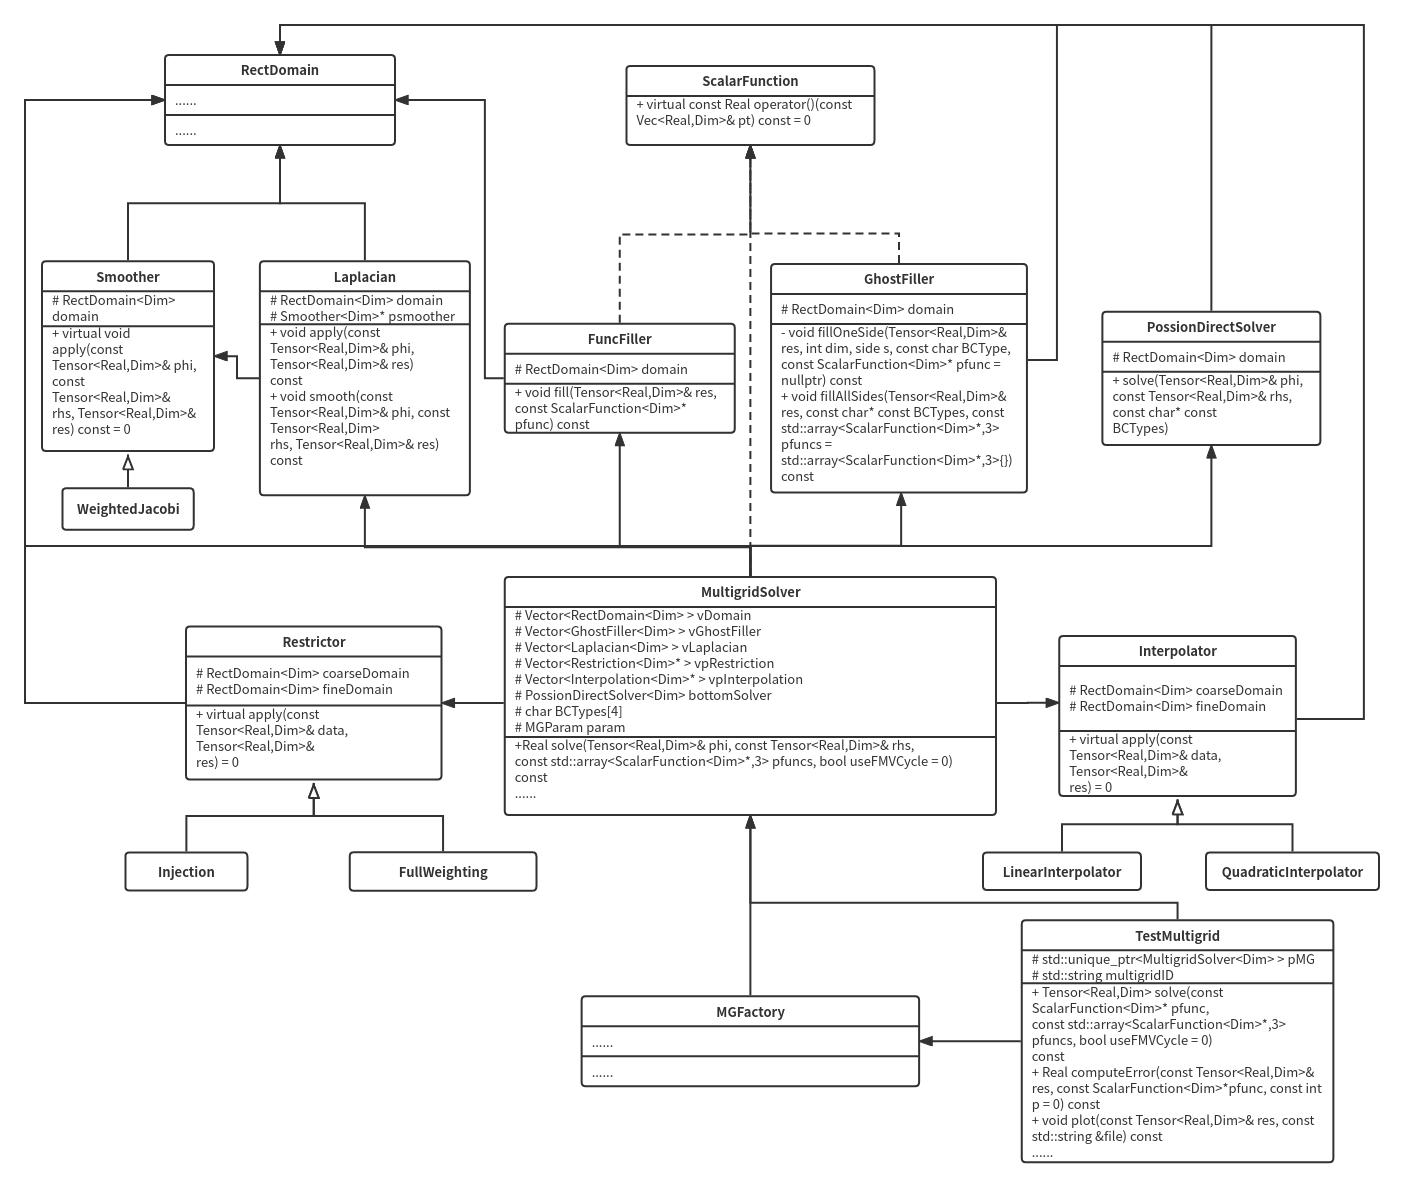
\includegraphics[width=16cm]{Multigrid2.png}                                           
  \caption{UML图}                        
\end{figure}
\end{document}


